\documentclass[11pt]{article}
\usepackage[T1]{fontenc}
\usepackage{lmodern}
\usepackage[margin=1in]{geometry}
\usepackage{amsmath,amssymb,amsthm}
\usepackage{microtype}
\usepackage{flafter}
\usepackage{enumitem}
\usepackage{tikz}
\usetikzlibrary{arrows.meta,positioning}
\usepackage[colorlinks=true,linkcolor=blue!45!black,citecolor=blue!45!black,urlcolor=blue!45!black]{hyperref}
\hypersetup{pdftitle={A superquadratic separation between sensitivity and block sensitivity},pdfauthor={OpenAI}}
\newcommand{\bs}{\operatorname{bs}}
\newcommand{\unverified}[1]{\par\smallskip\noindent\fbox{\parbox{0.95\linewidth}{\textbf{Unverified step.} #1}}\par\smallskip}
\newtheorem{theorem}{Theorem}[section]
\newtheorem{lemma}[theorem]{Lemma}
\newtheorem{proposition}[theorem]{Proposition}
\newtheorem{corollary}[theorem]{Corollary}
\theoremstyle{definition}
\newtheorem{definition}[theorem]{Definition}
\theoremstyle{remark}
\newtheorem{remark}[theorem]{Remark}
\title{A superquadratic separation between sensitivity\\and block sensitivity}
\author{Rewritten for readability from the OpenAI manuscript of the same title}
\date{September 25, 2026}
\begin{document}
\maketitle
\begin{abstract}
We disprove the quadratic strengthening of the Sensitivity Conjecture by
constructing nonconstant total Boolean functions whose block sensitivity grows
faster than any constant multiple of sensitivity squared. In fact, for some
fixed \(\alpha>2\), our examples have unbounded block sensitivity and satisfy
\(\bs(f)\ge s(f)^\alpha\).
\end{abstract}

\section{The result}
\label{sec:introduction}

\subsection{Definitions}
For a positive integer \(n\), write \([n]=\{1,\ldots,n\}\).
If \(x\in\{0,1\}^n\) and \(B\subseteq[n]\), let \(x^B\) be obtained from \(x\)
by flipping precisely the coordinates in \(B\); abbreviate \(x^{\{e\}}\) to
\(x^e\). All functions are \emph{total} Boolean functions
\(f:\{0,1\}^n\to\{0,1\}\). The \emph{sensitivity} of \(f\) is
\[
 s(f,x)=\bigl|\{e\in[n]:f(x^e)\ne f(x)\}\bigr|,
 \qquad s(f)=\max_x s(f,x).
\]
The \emph{block sensitivity} \(\bs(f,x)\) is the largest number of pairwise
disjoint nonempty sets \(B_1,\ldots,B_p\subseteq[n]\) such that
\(f(x^{B_j})\ne f(x)\) for every \(j\), and \(\bs(f)=\max_x\bs(f,x)\).
A set \(B\) with \(f(x^B)\ne f(x)\) is called a \emph{sensitive block} for \(f\)
at \(x\). Taking singleton blocks shows \(s(f,x)\le\bs(f,x)\).

\subsection{Main theorem}

\begin{theorem}\label{thm:main}
For every real \(C>0\), there are a positive integer \(n\) and a
nonconstant total Boolean function \(f:\{0,1\}^n\to\{0,1\}\) such that
\[
 \bs(f)>C\,s(f)^2.
\]
More precisely, for every integer \(d\ge1\) the construction below gives
a nonconstant total Boolean function \(f\) with
\[
 \frac{\bs(f)}{s(f)^2}\ge \frac{2^d}{4(d+2)^2}.
\]
\end{theorem}

The right-hand side first exceeds \(1\) at \(d=9\), where it equals
\(512/484=128/121\) (at \(d=8\) it is \(256/400\)). Section~\ref{sec:composition} uses the
\(d=9\) function as a seed and proves, by iterated composition, that there are
a fixed \(\alpha>2\) and functions \(F_m\) with
\(\bs(F_m,0)\ge s(F_m)^\alpha\) and \(\bs(F_m,0)\to\infty\)
(Corollary~\ref{cor:power-separation}).

\subsection{Context}
The Sensitivity Conjecture asked whether block sensitivity is bounded by a
polynomial in sensitivity, uniformly over the number of inputs and the
function. The question goes back to Nisan's work on parallel computation,
which introduced block sensitivity and already recorded Rubinstein's
quadratic separation \cite[Section~2]{Nisan1989}.
Nisan and Szegedy studied the problem through the degree of the unique
multilinear real polynomial representing a Boolean function, and explicitly
suggested the quadratic inequality \(\bs(f)\le s(f)^2\)
\cite[Section~4]{NisanSzegedy1994}.
Rubinstein's construction \cite{Rubinstein1995} showed that a polynomial
upper bound would need degree at least two. Virza improved the separation
to \(\bs(f)=\tfrac12s(f)^2+\tfrac12s(f)\) \cite{Virza2011}, and
Ambainis and Sun subsequently obtained examples satisfying
\(\bs(f)=\frac23s(f)^2-\frac13s(f)\)
\cite[Theorem~1]{AmbainisSun2011}.
These improvements left open whether any universal quadratic upper bound
could hold.

Huang resolved the polynomial conjecture in 2019. His degree bound,
together with Tal's refinement of the degree--block-sensitivity comparison
\cite{Tal2013}, gives \(\bs(f)\le s(f)^4\) for every total Boolean function
\cite[Theorem~1.5]{Huang2019}. Wellens later improved its leading constant,
proving \(\bs(f)\le\sqrt{2/3}\,s(f)^4+1\)
\cite[Corollary~4.2]{Wellens2022}.
These results settle the polynomial question; Theorem~\ref{thm:main} rules out
its quadratic strengthening.

\paragraph{Relation to spectral sensitivity.}
Meiburg's spectral-sensitivity construction uses tournament-indexed rows
of positive conditions and one selected blocking coordinate in each
outgoing row \cite[Sections~3.1 and~5.2--5.5]{Meiburg2026}.\footnote{In the
attribution accompanying this construction, Meiburg credits GPT-5.6-Sol
with the gated-tournament ideas and describes his own contributions as
exposition, size and parameter optimization, and checking the faithfulness
of the Lean formalization.}
There, random labels exclude small local configurations in which many accepting
subcubes lie close to the same accepting input. The present construction adapts this
architecture to nested predicates, using a different forbidden-label condition
and a direct union bound.
The sensitivity graph joins adjacent cube inputs exactly when the function
changes value. Its maximum degree is \(s(f)\); spectral sensitivity
\(\lambda(f)\) is the operator norm of its adjacency matrix
\cite{AaronsonEtAl2021}.
Since \(\lambda(f)\le s(f)\), a lower bound on
\(\bs(f)/\lambda(f)^2\) alone does not supply the ordinary-sensitivity
separation in Theorem~\ref{thm:main}. The estimates needed are proved directly
below, without a spectral input.

Two further ingredients are borrowed in spirit and reproved here. The final
OR of disjoint copies, which balances the sensitivities at zero and one, follows the principle used by
Ambainis and Sun \cite[Section~4, Lemma~1]{AmbainisSun2011}.
Ambainis and Pr\={u}sis explicitly noted that a seed with block sensitivity
greater than sensitivity squared would yield a superquadratic power separation
by iteration \cite[Section~1]{AmbainisPrusis2014}; composition as an
amplification method is treated systematically by Tal~\cite{Tal2013}.

\paragraph{Notation changes relative to the source.}
A single flipped coordinate is called \(e\) (the source uses \(a\), which
clashes with the edge labels \(a(i,j)\)). In the proof of
Proposition~\ref{prop:recurrences} the child thresholds are called
\(\gamma,\gamma'\) (source: \(g,g'\)) and the size of \(\mathcal G\) is called
\(w\) (source: \(m\)). In Lemma~\ref{lem:composition} the two input lengths are
\(n_1,n_2\) (source: \(a,b\)), the numbers of blocks are \(\mu,\nu\) (source:
\(p,q\)), and the blocks are \(Y_i,Z_j,W_{i,j}\) (source: \(C_i,D_j,E_{i,j}\)).
Lemma~\ref{lem:structure} collects facts that the source states in running text.

\section{Proof at a glance}
\label{sec:glance}

\paragraph{Key idea.}
We build, by a \(d\)-level recursion with a size parameter \(M\), a function
\(P_{d,1}\) that vanishes at the all-zero input. Each level multiplies the
number of pairwise disjoint sensitive blocks at zero by \(k=2M^2+1\), but
multiplies the sensitivity by only about \(M\). Since sensitivity is squared in
the ratio, each level gains a factor \(k/M^2\ge2\), for a total gain \(2^d\)
against a fixed loss \(4(d+2)^2\).

\paragraph{One level of the recursion.}
The input is cut into \(k\) rows of \(r=\lceil\sqrt M\rceil\) disjoint child
inputs. The rows are the vertices of a tournament in which every vertex has
outdegree \(M^2\), and each edge \(i\to j\) carries a label
\(a(i,j)\in[r]\) pointing at one child of row \(j\). At the previous level we
have not one function but a \emph{nested} family
\(P_{\ell-1,1}\ge P_{\ell-1,2}\ge\cdots\). Clause \(i\) says: the strongest
child predicate accepts all \(r\) children of row \(i\) (\emph{targets}), and
for every edge \(i\to j\) a weaker child predicate rejects the labelled child
of row \(j\) (\emph{gates}). The parent predicate is the OR of the \(k\)
clauses. Varying which weaker predicate the gates use gives the nested family
at the next level.

\paragraph{Why sensitivity stays small.}
Let \(S_{\ell,b}\) be the largest number of single-bit flips that move a
level-\(\ell\) predicate from value \(b\) to \(1-b\).
\begin{itemize}[leftmargin=2em]
\item \emph{At a one-input} one satisfied clause must be broken. It has \(M^2\) gates
and \(r\) targets, each on a different child, so
\(S_{\ell,1}\le M^2S_{\ell-1,0}+rS_{\ell-1,1}\).
\item \emph{At a zero-input} a single flip touches one child, hence one
condition per clause, so only clauses with \emph{exactly one} failed condition
can become satisfied. If the failed condition is a target, the labelling
(Lemma~\ref{lem:labelling}) allows fewer than \(16\) such clauses. If it is a gate,
the tournament allows at most \(3\) such clauses, and for all but at most one
of them the failed gate sits on a child accepted by the strongest predicate.
Repairing such a gate forces \emph{two different} child predicates to drop from one to
zero under the same flip.
\end{itemize}
We therefore also track \(J_{\ell,b}\), the largest number of flips that move
a fixed pair of distinct predicates from \(b\) to \(1-b\) simultaneously.
The outcome (Proposition~\ref{prop:recurrences}) is
\(S_{\ell,0}\le 16\,S_{\ell-1,0}+S_{\ell-1,1}+3J_{\ell-1,1}\).
The coefficient of \(S_{\ell-1,1}\) is \(1\), not \(3\).
The joint profiles start at zero, because the level-\(0\) predicates are Hamming
balls of consecutive integer radii and one flip cannot cross two radii
(Lemma~\ref{lem:base}). They then stay negligible if \(M\ge9^{d+1}\)
(Lemma~\ref{lem:quantitative-profiles}).

\paragraph{Steps and dependencies.}
\begin{enumerate}[leftmargin=2em]
\item Lemma~\ref{lem:labelling}: a labelling with no ``consistent'' \(16\)-set
exists (union bound).
\item Lemma~\ref{lem:structure}: nesting, and ``one flip changes at most one
condition per clause''.
\item Lemma~\ref{lem:base}: level-\(0\) profiles \(S_{0,0}\le L\),
\(S_{0,1}\le LM\), \(J_{0,b}=0\).
\item Lemma~\ref{lem:blocks}: \(Mk^\ell\) disjoint sensitive blocks at zero.
\item Proposition~\ref{prop:recurrences}: four recurrences for
\(S_{\ell,b},J_{\ell,b}\) (uses 1 and 2).
\item Lemma~\ref{lem:quantitative-profiles}:
\(S_{\ell,b}\le2LM^{\ell+b}\) when \(M\ge9^{d+1}\) (uses 3 and 5).
\item Theorem~\ref{thm:main}: \(f\) is the OR of \(M\) disjoint copies of
\(P_{d,1}\), so that \(s(f)\le 2LM^{d+1}\) and \(\bs(f,0)\ge M^2k^d\) (uses 4 and 6).
\item Lemma~\ref{lem:composition} and Corollary~\ref{cor:power-separation}:
composition turns the \(d=9\) seed into a fixed exponent \(\alpha>2\) (uses the
two bounds of step 7).
\end{enumerate}

\begin{figure}[htbp]
\centering
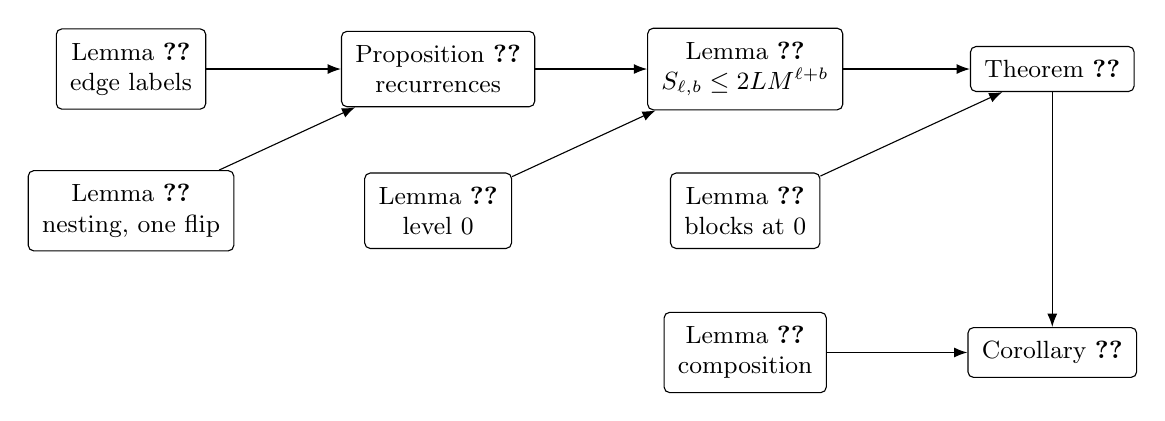
\begin{tikzpicture}[>=Latex, every node/.style={font=\small},
  box/.style={draw,rounded corners=2pt,inner sep=5pt,align=center}]
 \node[box] (lab) at (0,1.8) {Lemma~\ref{lem:labelling}\\edge labels};
 \node[box] (str) at (0,0) {Lemma~\ref{lem:structure}\\nesting, one flip};
 \node[box] (rec) at (3.9,1.8) {Proposition~\ref{prop:recurrences}\\recurrences};
 \node[box] (base) at (3.9,0) {Lemma~\ref{lem:base}\\level \(0\)};
 \node[box] (quant) at (7.8,1.8) {Lemma~\ref{lem:quantitative-profiles}\\\(S_{\ell,b}\le2LM^{\ell+b}\)};
 \node[box] (blk) at (7.8,0) {Lemma~\ref{lem:blocks}\\blocks at \(0\)};
 \node[box] (main) at (11.7,1.8) {Theorem~\ref{thm:main}};
 \node[box] (comp) at (7.8,-1.8) {Lemma~\ref{lem:composition}\\composition};
 \node[box] (cor) at (11.7,-1.8) {Corollary~\ref{cor:power-separation}};
 \draw[->] (lab) -- (rec);
 \draw[->] (str) -- (rec);
 \draw[->] (base) -- (quant);
 \draw[->] (rec) -- (quant);
 \draw[->] (quant) -- (main);
 \draw[->] (blk) -- (main);
 \draw[->] (main) -- (cor);
 \draw[->] (comp) -- (cor);
\end{tikzpicture}
\caption{Logical dependencies.}
\label{fig:dependencies}
\end{figure}

\section{The labelled tournament and nested predicates}
\label{sec:construction}

\subsection{Parameters and the tournament}
Fix integers \(d\ge1\) and \(M\ge3\), and put
\[
 L=d+2,\qquad k=2M^2+1,\qquad r=\lceil\sqrt M\rceil,
 \qquad t=16.
\]
The construction is defined for every \(M\ge3\); only
Section~\ref{sec:separation} requires \(M\ge9^{d+1}\).

A \emph{tournament} on a vertex set is an orientation of every pair of distinct
vertices: exactly one of \(i\to j\) and \(j\to i\) holds.
Fix a tournament on \([k]\) in which every vertex has outdegree \(M^2\).
One exists: place the \(k=2M^2+1\) vertices cyclically and direct an edge from
each vertex to the next \(M^2\) vertices. For \(i\ne j\), exactly one of
\(j-i\) and \(i-j\) is congruent modulo \(k\) to an element of
\(\{1,\ldots,M^2\}\), so this is a tournament.

\subsection{Edge labels}
The tournament rows and selected blocking coordinates adapt the architecture
of Meiburg~\cite[Sections~3.1 and~5.2--5.5]{Meiburg2026}. The following label
property is used once, in Step~4 of the proof of
Proposition~\ref{prop:recurrences}, to bound the number of clauses that are one
target short of being satisfied.

\begin{lemma}\label{lem:labelling}
The edges can be labelled by numbers \(a(i,j)\in[r]\) so that there is
no set \(I\subseteq[k]\) of size \(t\) admitting choices
\(m_j\in[r]\), \(j\in I\), with
\[
 a(i,j)=m_j \qquad\text{for every edge }i\to j\text{ within }I.
\]
\end{lemma}
\begin{proof}
Choose all edge labels independently and uniformly from \([r]\).

\emph{One bad configuration.} Fix \(I\) with \(|I|=t=16\) and fix
\((m_j)_{j\in I}\). The tournament has exactly one edge for each of the
\(\binom{16}{2}=120\) pairs in \(I\). The event in the lemma prescribes the
label of each of these \(120\) edges, so by independence it has probability
\(r^{-120}\).

\emph{Union bound.} There are at most \(k^{16}\) sets \(I\) and \(r^{16}\)
tuples \((m_j)\). Using \(k=2M^2+1\le3M^2\), \(r\ge\sqrt M\) and \(M\ge3\),
the probability that some bad configuration occurs is at most
\[
 k^{16}r^{16}r^{-120}=k^{16}r^{-104}\le (3M^2)^{16}(\sqrt M)^{-104}
 =3^{16}M^{32-52}=3^{16}M^{-20}\le 3^{-4}<1.
\]
Hence some labelling has no bad configuration.
\end{proof}

Fix such a labelling for the remainder of the construction.

\subsection{The predicates}
For \(0\le\ell\le d\), set
\[
 H_\ell=d+1-\ell,\qquad N_\ell=LM(kr)^\ell.
\]
We define predicates \(P_{\ell,q}:\{0,1\}^{N_\ell}\to\{0,1\}\) for
\(1\le q\le H_\ell\). At level \(d\) there is a single predicate \(P_{d,1}\),
since \(H_d=1\).

\paragraph{Level \(0\).}
Partition \([LM]\) into \(M\) blocks \(E_1,\ldots,E_M\), each of
size \(L\). Let \(z_j\in\{0,1\}^{LM}\) be the string that is one precisely on
\(E_j\). Write \(\operatorname{dist}\) for Hamming distance and set
\[
 D(x)=\min_{j\in[M]}\operatorname{dist}(x,z_j),\qquad
 P_{0,q}(x)=\mathbf1\{D(x)\le H_0-q\}\quad(1\le q\le H_0=d+1).
\]
So \(P_{0,q}\) is the indicator of the union of the Hamming balls of radius
\(d+1-q\) around the centres \(z_j\). The radii are the integers from \(d\)
down to \(0\). Distinct centres have disjoint supports of size \(L\), hence
distance \(2L=2d+4\).

\paragraph{Level \(\ell\), \(1\le\ell\le d\).}
Partition the \(N_\ell=kr\,N_{\ell-1}\) input bits into \(kr\) disjoint
\emph{children} \(x_{j,c}\in\{0,1\}^{N_{\ell-1}}\), arranged in \(k\) rows
\(j\in[k]\), each with \(r\) positions \(c\in[r]\).
Put \(H=H_\ell\) and \(Q=H+1=H_{\ell-1}\).
For \(q\in[H]\) and \(i\in[k]\), \emph{clause \(i\) at index \(q\)} asserts
\begin{equation}\label{eq:predicate-definition}
 \begin{aligned}
 P_{\ell-1,Q}(x_{i,c})&=1 &&\text{for all }c\in[r],\\
 P_{\ell-1,Q-q}(x_{j,a(i,j)})&=0 &&\text{for all }j\text{ with }i\to j.
 \end{aligned}
\end{equation}
The first line consists of the \(r\) \emph{target conditions} and the second of the
\(M^2\) \emph{gate conditions} (Figure~\ref{fig:clause}). Define
\(P_{\ell,q}(x)=1\) if at least one of the \(k\) clauses at index \(q\) is
satisfied, and \(P_{\ell,q}(x)=0\) otherwise. The indices are valid: for
\(q\in[H]\) we have \(1\le Q-q\le H<Q=H_{\ell-1}\). The targets do not depend
on \(q\); only the gates do.

\begin{figure}[htbp]
\centering
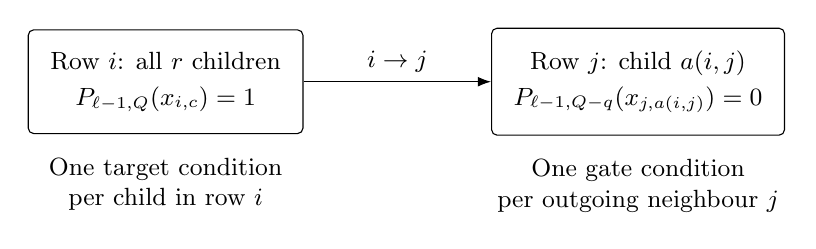
\begin{tikzpicture}[>=Latex, every node/.style={font=\small},
  condition/.style={draw,rounded corners=2pt,inner sep=8pt,align=center}]
 \node[condition] (target) at (0,0)
   {Row \(i\): all \(r\) children\\[2pt]
    \(P_{\ell-1,Q}(x_{i,c})=1\)};
 \node[condition] (gate) at (6,0)
   {Row \(j\): child \(a(i,j)\)\\[2pt]
    \(P_{\ell-1,Q-q}(x_{j,a(i,j)})=0\)};
 \draw[->] (target) -- node[above]{\(i\to j\)} (gate);
 \node[below=5pt of target,align=center] {One target condition\\per child in row \(i\)};
 \node[below=5pt of gate,align=center] {One gate condition\\per outgoing neighbour \(j\)};
\end{tikzpicture}
\caption{One recursive clause. The edge label selects a single child in
each outgoing neighbour's row. Raising \(q\) strengthens the gates;
all targets use the strongest child predicate \(Q\).}
\label{fig:clause}
\end{figure}

\subsection{Structural facts}
The next lemma is used throughout Proposition~\ref{prop:recurrences}; part (a)
is also what ``nested'' means. Nesting concerns the predicate index, not the
input bits.

\begin{lemma}\label{lem:structure}
Let \(0\le\ell\le d\).
\begin{enumerate}[label=\textup{(\alph*)},leftmargin=2.2em]
\item \textup{(Nesting.)} For \(1\le p<p'\le H_\ell\) and every \(x\),
\(P_{\ell,p}(x)\ge P_{\ell,p'}(x)\). Equivalently: a one at the larger index
\(p'\) forces a one at the smaller index \(p\), and a zero at \(p\) forces a
zero at \(p'\).
\end{enumerate}
Now let \(\ell\ge1\).
\begin{enumerate}[label=\textup{(\alph*)},leftmargin=2.2em,resume]
\item \textup{(Clauses are nested.)} If \(q<q'\) and clause \(i\) at index
\(q'\) is satisfied at \(x\), then clause \(i\) at index \(q\) is satisfied at
\(x\).
\item \textup{(Distinct children.)} For fixed \(i\) and \(q\), the \(r+M^2\)
conditions of clause \(i\) at index \(q\) refer to \(r+M^2\) distinct children.
\item \textup{(One flip, one condition.)} Let \(e\in[N_\ell]\). The inputs
\(x\) and \(x^e\) differ in exactly one child, namely the one containing \(e\).
Hence, for fixed \(i\) and \(q\), at most one condition of clause \(i\) at
index \(q\) has different truth values at \(x\) and \(x^e\), and such a
condition refers to the child containing \(e\).
\end{enumerate}
\end{lemma}
\begin{proof}
(a) and (b), by induction on \(\ell\). At level \(0\), if \(p<p'\) then
\(D(x)\le H_0-p'\) implies \(D(x)\le H_0-p\), which is (a).
Let \(\ell\ge1\) and assume (a) at level \(\ell-1\). Suppose clause \(i\) at
index \(q'\) is satisfied at \(x\), and \(q<q'\). The targets of the two
clauses are identical. For each gate,
\(P_{\ell-1,Q-q'}(x_{j,a(i,j)})=0\). Since \(Q-q'<Q-q\), part (a) at level
\(\ell-1\) (a zero at the smaller index forces a zero at the larger) gives
\(P_{\ell-1,Q-q}(x_{j,a(i,j)})=0\). So clause \(i\) at index \(q\) is
satisfied; this is (b). If \(P_{\ell,q'}(x)=1\), some clause at index \(q'\)
is satisfied, hence so is the same clause at index \(q\), and
\(P_{\ell,q}(x)=1\); this is (a) at level \(\ell\).

(c) The targets use the \(r\) children \((i,c)\), \(c\in[r]\), all in row
\(i\). Each gate uses a child in a row \(j\ne i\), and there is exactly one
gate for each out-neighbour \(j\), so different gates use different rows.

(d) The children partition the coordinates, so \(e\) lies in exactly one child
and the other children are identical in \(x\) and \(x^e\). A condition is a
statement about a single child, so by (c) at most one condition of the clause
can change.
\end{proof}

The same bit can affect several clauses. This causes no problem, because every
count below is an upper bound on a union of sets of bits.

\subsection{Sensitivity profiles and the level-\(0\) bounds}
For \(b\in\{0,1\}\) and \(0\le\ell\le d\), define the \emph{ordinary profile}
\[
 S_{\ell,b}=\max_{\substack{1\le q\le H_\ell,\ x\in\{0,1\}^{N_\ell}\\
                           P_{\ell,q}(x)=b}}
 \bigl|\{e\in[N_\ell]:P_{\ell,q}(x^e)=1-b\}\bigr|
\]
and the \emph{joint profile}
\[
 J_{\ell,b}=\max_{\substack{1\le q<q'\le H_\ell,\ x\in\{0,1\}^{N_\ell}\\
                         P_{\ell,q}(x)=P_{\ell,q'}(x)=b}}
 \bigl|\{e\in[N_\ell]:P_{\ell,q}(x^e)=P_{\ell,q'}(x^e)=1-b\}\bigr|.
\]
In \(J_{\ell,b}\) the two predicates are evaluated on the same input and
changed by the same bit. A maximum over no cases is defined to be zero; in
particular \(J_{d,0}=J_{d,1}=0\), since \(H_d=1\).

The next lemma supplies the initial values for the induction in
Lemma~\ref{lem:quantitative-profiles}.

\begin{lemma}\label{lem:base}
The initial sensitivity profiles satisfy
\begin{equation}\label{eq:base-profile}
 S_{0,0}\le L,\qquad S_{0,1}\le LM,\qquad
 J_{0,0}=J_{0,1}=0.
\end{equation}
\end{lemma}
\begin{proof}
\emph{Preliminary.} For adjacent inputs \(x,y\) (differing in one bit) and
every \(j\), the triangle inequality gives
\(\operatorname{dist}(x,z_j)\le\operatorname{dist}(y,z_j)+1\), so
\(D(x)\le D(y)+1\). By symmetry, \(|D(x)-D(y)|\le1\).

\emph{\(S_{0,0}\le L\).} Fix \(q\), put \(R=H_0-q\in\{0,\ldots,d\}\), and let
\(x\) satisfy \(P_{0,q}(x)=0\), that is, \(D(x)\ge R+1\). Suppose
\(P_{0,q}(x^e)=1\). Then some centre \(z_j\) has
\(\operatorname{dist}(x^e,z_j)\le R\), so
\(\operatorname{dist}(x,z_j)\le R+1\). Combined with \(D(x)\ge R+1\) this gives
\(\operatorname{dist}(x,z_j)=R+1\) and \(\operatorname{dist}(x^e,z_j)=R\), so
\(e\) is one of the \(R+1\) coordinates where \(x\) and \(z_j\) differ.
The centre \(z_j\) is the same for all such \(e\). Indeed, it lies within distance
\(R+1\le d+1\) of \(x\), and two distinct centres within distance \(d+1\) of
\(x\) would be at distance at most \(2d+2<2d+4=2L\) from each other,
contradicting the fact that distinct centres are at distance \(2L\). Hence
there are at most \(R+1\le d+1\le L\) such coordinates \(e\).

\emph{\(S_{0,1}\le LM\).} This is the total number \(N_0=LM\) of input bits.

\emph{\(J_{0,b}=0\).} Let \(q<q'\), with radii \(R=H_0-q>R'=H_0-q'\).
If one flip took both predicates from zero to one, then \(D(x)\ge R+1\) and
\(D(x^e)\le R'\le R-1\). If it took both from one to zero, then
\(D(x)\le R'\) and \(D(x^e)\ge R+1\ge R'+2\). Either way \(D\) changes by at
least two, contradicting the preliminary.
\end{proof}

\subsection{Disjoint blocks at zero}
The next lemma gives the block-sensitivity lower bound in the proof of
Theorem~\ref{thm:main}. It concerns only the all-zero input; the sensitivity
upper bounds of Section~\ref{sec:recurrences} hold at every input.

\begin{lemma}\label{lem:blocks}
At every level \(0\le\ell\le d\), all predicates are zero at the
all-zero input. There are \(Mk^\ell\) pairwise disjoint nonempty blocks
of coordinates, each of size \(Lr^\ell\), such that flipping any one
block at zero makes every predicate at that level equal to one.
\end{lemma}
\begin{proof}
Induction on \(\ell\).

\emph{Level \(0\).} Every centre has weight \(L\), so \(D(0)=L>d\), and every
radius is at most \(d\); hence \(P_{0,q}(0)=0\) for all \(q\). The \(M\)
blocks \(E_j\) of size \(L\) work: \(0^{E_j}=z_j\) has \(D=0\), so every
\(P_{0,q}\) is one there.

\emph{Level \(\ell\ge1\), assuming level \(\ell-1\).}
At the all-zero input every child is all-zero, so by induction the target
predicate \(P_{\ell-1,Q}\) is zero on every child. Every clause has at least
one target, so every clause fails, and \(P_{\ell,q}(0)=0\) for all \(q\).

Let \(B_1,\ldots,B_{Mk^{\ell-1}}\) be the block family at level \(\ell-1\).
For each row \(i\in[k]\) and each \(h\), let \(B_{i,h}\) be the union of the
copies of \(B_h\) in the \(r\) children of row \(i\). After flipping
\(B_{i,h}\) at zero:
\begin{itemize}[leftmargin=2em]
\item each child of row \(i\) equals \(0^{B_h}\), on which every
level-\((\ell-1)\) predicate, in particular \(P_{\ell-1,Q}\), is one, so all
targets of clause \(i\) hold;
\item every gate child of clause \(i\) lies in another row and is still
all-zero, so \(P_{\ell-1,Q-q}\) is zero there by induction, and all gates
of clause \(i\) hold for every \(q\).
\end{itemize}
Thus clause \(i\) is satisfied at every index, and every \(P_{\ell,q}\) is one.
The sets \(B_{i,h}\) are pairwise disjoint: for different rows they lie in
different children, and for the same row and different \(h\) they are disjoint
inside each child. There are \(k\cdot Mk^{\ell-1}=Mk^\ell\) of them, each of
size \(r\cdot Lr^{\ell-1}=Lr^\ell\).
\end{proof}

As a consistency check, \(Mk^\ell\cdot Lr^\ell=N_\ell\), so the blocks
partition the whole input.

\section{Sensitivity recurrences}
\label{sec:recurrences}

This proposition is the core of the argument. It feeds
Lemma~\ref{lem:quantitative-profiles}.

\begin{proposition}\label{prop:recurrences}
For $1\leq \ell\leq d$, write
$S'_b=S_{\ell-1,b}$ and $J'_b=J_{\ell-1,b}$.  Then
\begin{equation}\label{eq:recurrences}
\begin{aligned}
 S_{\ell,1}&\leq M^2S'_0+rS'_1,
 &\qquad J_{\ell,1}&\leq M^2J'_0+rS'_1,\\
 S_{\ell,0}&\leq tS'_0+S'_1+3J'_1,
 &\qquad J_{\ell,0}&\leq tS'_0+3J'_1.
\end{aligned}
\end{equation}
\end{proposition}

\paragraph{Plan.}
In each of the four cases we fix the input \(x\) and the parent index (or pair
of indices), and cover the set of ``successful'' flips \(e\) by a union of
sets, each consisting of flips inside one specific child that change one
specific child predicate (or pair of child predicates) in a specific
direction. Each such set is bounded by a child profile. On the one side the
relevant children are those of one fixed satisfied clause. On the zero side
they are the children of the unique failed conditions of a short list of
candidate clauses.

\begin{proof}
\emph{Standing notation.} Fix \(\ell\), put \(H=H_\ell\), \(Q=H+1\), and
abbreviate \(P'_p=P_{\ell-1,p}\) for \(p\in[Q]\). A child is a pair
\(\kappa=(j,c)\in[k]\times[r]\) with input \(x_\kappa\). If the coordinate
\(e\) lies in child \(\kappa\), then \((x^e)_\kappa\) is \(x_\kappa\) with one
bit flipped, and all other children are unchanged. We make no restriction on
how many of the predicates \(P'_p\) of that child the flip changes. Applying
the definitions of \(S'_b\) and \(J'_b\) to the level-\((\ell-1)\) input
\(x_\kappa\) gives two counting facts.
\begin{itemize}[leftmargin=3em]
\item[(C1)] If \(P'_p(x_\kappa)=b\), at most \(S'_b\) coordinates \(e\) of
child \(\kappa\) satisfy \(P'_p((x^e)_\kappa)=1-b\).
\item[(C2)] If \(p<p'\) and \(P'_p(x_\kappa)=P'_{p'}(x_\kappa)=b\), at most
\(J'_b\) coordinates \(e\) of child \(\kappa\) satisfy
\(P'_p((x^e)_\kappa)=P'_{p'}((x^e)_\kappa)=1-b\).
\end{itemize}

\medskip\noindent\textbf{Step 1: \(S_{\ell,1}\le M^2S'_0+rS'_1\).}
Fix \(q\in[H]\) and \(x\) with \(P_{\ell,q}(x)=1\), and fix one clause \(i\)
(at index \(q\)) satisfied at \(x\). Let \(e\) be a flip with
\(P_{\ell,q}(x^e)=0\). Then clause \(i\) is not satisfied at \(x^e\), so one
of its conditions is true at \(x\) and false at \(x^e\). By
Lemma~\ref{lem:structure}(d), \(e\) lies in the child of that condition.
\begin{itemize}[leftmargin=2em]
\item If it is a target, on child \((i,c)\), then \(P'_Q\) changes from one to
zero there. By (C1) each of the \(r\) target children accounts for at most
\(S'_1\) flips.
\item If it is a gate, on child \((j,a(i,j))\), then \(P'_{Q-q}\) changes from
zero to one there. By (C1) each of the \(M^2\) gate children accounts for at
most \(S'_0\) flips.
\end{itemize}
So at most \(M^2S'_0+rS'_1\) flips take \(P_{\ell,q}\) to zero.

\medskip\noindent\textbf{Step 2: \(J_{\ell,1}\le M^2J'_0+rS'_1\).}
Fix \(q<q'\) in \([H]\) and \(x\) with
\(P_{\ell,q}(x)=P_{\ell,q'}(x)=1\). Fix a clause \(i\) satisfied at \(x\) at
index \(q'\). By Lemma~\ref{lem:structure}(b) it is also satisfied at index
\(q\). Put
\[
 \gamma=Q-q,\qquad \gamma'=Q-q',\qquad 1\leq \gamma'<\gamma<Q.
\]
Let \(e\) be a flip with \(P_{\ell,q}(x^e)=P_{\ell,q'}(x^e)=0\). In particular
clause \(i\) at index \(q\) is not satisfied at \(x^e\), so one of its
conditions at index \(q\) is true at \(x\) and false at \(x^e\), and \(e\)
lies in its child \(\kappa\).
\begin{itemize}[leftmargin=2em]
\item If it is a target, then as in Step 1 there are at most \(rS'_1\) such
flips in total.
\item If it is a gate, on \(\kappa=(j,a(i,j))\), then at \(x\) we have
\(P'_{\gamma'}(x_\kappa)=0\), because clause \(i\) holds at index \(q'\), and
\(P'_{\gamma}(x_\kappa)=0\), because it holds at index \(q\). At \(x^e\) the
gate at index \(q\) fails, so \(P'_\gamma((x^e)_\kappa)=1\), and nesting
(Lemma~\ref{lem:structure}(a), \(\gamma'<\gamma\)) gives
\(P'_{\gamma'}((x^e)_\kappa)=1\). Thus the two distinct child predicates
\(P'_{\gamma'},P'_\gamma\) both change from zero to one. By (C2) each of the
\(M^2\) gate children accounts for at most \(J'_0\) flips.
\end{itemize}
So at most \(M^2J'_0+rS'_1\) flips take both predicates to zero.

\medskip\noindent\textbf{Step 3: candidate clauses at a zero.}
Fix \(q\in[H]\) and \(x\) with \(P_{\ell,q}(x)=0\). In Steps 3--6 all clauses
are at index \(q\). Let
\begin{align*}
\mathcal T&=\{i\in[k]:\text{at }x\text{, clause }i\text{ fails exactly one target and no gate}\},\\
\mathcal G&=\{i\in[k]:\text{at }x\text{, clause }i\text{ fails exactly one gate and no target}\}.
\end{align*}
These sets depend only on \(x\) and \(q\), not on any flip. For
\(i\in\mathcal T\cup\mathcal G\), let \(\kappa_i\) be the child of the unique
failed condition of clause \(i\).

\emph{Claim.} If a clause \(i\) is satisfied at \(x^e\), then
\(i\in\mathcal T\cup\mathcal G\), the coordinate \(e\) lies in \(\kappa_i\),
and the unique failed condition of clause \(i\) is true at \(x^e\).

\emph{Proof of the claim.} Since \(P_{\ell,q}(x)=0\), clause \(i\) is not
satisfied at \(x\). By Lemma~\ref{lem:structure}(d) at most one of its
conditions differs between \(x\) and \(x^e\), and all are true at \(x^e\).
Hence exactly one condition fails at \(x\), it is repaired by the flip, and
\(e\) lies in its child.

In particular, every \(e\) with \(P_{\ell,q}(x^e)=1\) repairs the unique failed
condition of some clause in \(\mathcal T\cup\mathcal G\).

\medskip\noindent\textbf{Step 4: \(|\mathcal T|<t\).}
For \(j\in\mathcal T\), let \(m_j\in[r]\) be the position of its unique failed
target, so that \(P'_Q(x_{j,c})=0\) exactly for \(c=m_j\). Let
\(i,j\in\mathcal T\) with \(i\to j\). Clause \(i\) fails no gate, so
\(P'_{Q-q}(x_{j,a(i,j)})=0\). By nesting (\(Q-q<Q\); a zero at the smaller
index forces a zero at the larger), \(P'_Q(x_{j,a(i,j)})=0\). So the target of
clause \(j\) at position \(a(i,j)\) fails, and therefore \(a(i,j)=m_j\).
If \(|\mathcal T|\ge t\), any \(t\)-subset \(I\subseteq\mathcal T\) with these
\(m_j\) would violate Lemma~\ref{lem:labelling}. Hence
\(|\mathcal T|\le t-1\).

\medskip\noindent\textbf{Step 5: \(|\mathcal G|\le3\), and at most one vertex of
\(\mathcal G\) has no out-neighbour in \(\mathcal G\).}
Let \(i,j\in\mathcal G\) with \(i\to j\). Clause \(j\) fails no target, so
\(P'_Q(x_{j,c})=1\) for all \(c\), in particular for \(c=a(i,j)\). By nesting
(a one at the larger index \(Q\) forces a one at the smaller index \(Q-q\)),
\(P'_{Q-q}(x_{j,a(i,j)})=1\). That is, the gate of clause \(i\) for the edge
\(i\to j\) fails. Since clause \(i\) has exactly one failed gate, every vertex
has outdegree at most one in the tournament induced on \(\mathcal G\).
With \(w=|\mathcal G|\), counting the edges of the induced tournament by their tails
gives
\[
 \frac{w(w-1)}2\leq w,
 \qquad\text{and hence}\qquad w\leq3.
\]
Moreover, any two vertices of \(\mathcal G\) are joined by an edge that leaves
one of them, so at most one vertex of \(\mathcal G\) has outdegree zero in the
induced tournament.

\medskip\noindent\textbf{Step 6: \(S_{\ell,0}\le tS'_0+S'_1+3J'_1\).}
For \(i\in\mathcal T\cup\mathcal G\), let \(R_i\) be the set of coordinates
\(e\) in child \(\kappa_i\) such that the unique failed condition of clause
\(i\) is true at \(x^e\). By Step 3,
\(\{e:P_{\ell,q}(x^e)=1\}\subseteq\bigcup_{i\in\mathcal T\cup\mathcal G}R_i\).
We bound \(|R_i|\) in three cases.
\begin{itemize}[leftmargin=2em]
\item \(i\in\mathcal T\). The failed target has \(P'_Q(x_{\kappa_i})=0\), and
a repair makes it one. By (C1), \(|R_i|\le S'_0\).
\item \(i\in\mathcal G\) with an out-neighbour \(j\in\mathcal G\). By Step 5
the gate for \(i\to j\) is the unique failed gate, so
\(\kappa_i=(j,a(i,j))\), and
\[
 P'_{Q-q}(x_{\kappa_i})=P'_Q(x_{\kappa_i})=1 .
\]
A repair sets \(P'_{Q-q}((x^e)_{\kappa_i})=0\), and nesting then forces
\(P'_Q((x^e)_{\kappa_i})=0\). The indices \(Q-q<Q\) are distinct because
\(q\ge1\), so both of two distinct child predicates change from one to zero.
By (C2), \(|R_i|\le J'_1\). Such a flip also breaks a target of clause \(j\).
That is irrelevant: we are bounding a set of flips from above, and the
witness is clause \(i\), whose targets and other gates lie in other children.
\item \(i\in\mathcal G\) with no out-neighbour in \(\mathcal G\). The failed
gate has \(P'_{Q-q}(x_{\kappa_i})=1\), and a repair makes it zero. By (C1),
\(|R_i|\le S'_1\).
\end{itemize}
By Step 4 the first case contributes at most \((t-1)S'_0\le tS'_0\). By Step 5
there are at most three clauses in \(\mathcal G\), and at most one of them is in the third
case, so \(\mathcal G\) contributes at most \(S'_1+3J'_1\). Summing gives the
bound.

\medskip\noindent\textbf{Step 7: \(J_{\ell,0}\le tS'_0+3J'_1\).}
Fix \(q<q'\) in \([H]\) and \(x\) with
\(P_{\ell,q}(x)=P_{\ell,q'}(x)=0\). Form \(\mathcal T,\mathcal G,\kappa_i,R_i\)
as in Steps 3--6 for the \emph{smaller} index \(q\); those steps used only
\(P_{\ell,q}(x)=0\). Put \(\gamma=Q-q\) and \(\gamma'=Q-q'\), so
\(1\le\gamma'<\gamma<Q\).

Let \(e\) be a flip with \(P_{\ell,q}(x^e)=P_{\ell,q'}(x^e)=1\). Choose a
clause \(i\) satisfied at \(x^e\) at index \(q'\). This choice may depend on
\(e\), whereas the lists do not. By Lemma~\ref{lem:structure}(b), clause \(i\) is
also satisfied at \(x^e\) at index \(q\). The claim of Step 3 gives
\(i\in\mathcal T\cup\mathcal G\) and \(e\in R_i\).
\begin{itemize}[leftmargin=2em]
\item If \(i\in\mathcal T\), then \(e\in R_i\) with \(|R_i|\le S'_0\) as in
Step 6. Over all \(i\in\mathcal T\) this is at most \(tS'_0\).
\item If \(i\in\mathcal G\), let \(\kappa=\kappa_i\) be the child of its
unique failed gate at index \(q\). At \(x\) the gate fails, so
\(P'_\gamma(x_\kappa)=1\), and nesting gives \(P'_{\gamma'}(x_\kappa)=1\).
At \(x^e\) clause \(i\) holds at index \(q'\), and its gate at index \(q'\)
on the same edge refers to the same child \(\kappa\). So
\(P'_{\gamma'}((x^e)_\kappa)=0\), and nesting gives
\(P'_\gamma((x^e)_\kappa)=0\). Thus the two distinct child predicates
\(P'_{\gamma'},P'_\gamma\) both change from one to zero, and by (C2) at most
\(J'_1\) flips \(e\) arise from this \(i\). This argument does not use the
value of \(P'_Q\) on \(\kappa\), so it applies to every \(i\in\mathcal G\),
including the possible vertex with no out-neighbour in \(\mathcal G\): the
second parent index supplies the second child threshold. With
\(|\mathcal G|\le3\) the total is at most \(3J'_1\).
\end{itemize}
Every joint-success flip is counted in one of the two cases, so there are at most
\(tS'_0+3J'_1\) of them. (We never needed candidate lists for the index
\(q'\): a member of the lists for \(q\) that cannot be satisfied at index
\(q'\) after one flip simply contributes nothing.)

\medskip\noindent\textbf{Step 8: conclusion.}
Steps 1, 2, 6 and 7 hold for every admissible input and every index or pair of
indices, so taking maxima gives \eqref{eq:recurrences}. If \(H=1\) there is no
pair \(q<q'\), and the two joint inequalities hold by the empty-maximum
convention.
\end{proof}

\section{Quantitative bounds and separation}
\label{sec:separation}

The dominant terms \(M^2S'_0\) and \(S'_1\) in
Proposition~\ref{prop:recurrences} suggest normalizing \(S_{\ell,b}\) by
\(M^{\ell+b}\). The joint profiles vanish at level \(0\); choosing \(M\) large
relative to \(d\) keeps their contribution small through depth \(d\). The next
lemma is the sensitivity input to the proof of Theorem~\ref{thm:main}.

\begin{lemma}
\label{lem:quantitative-profiles}
Suppose that $d\geq 1$ and $M\geq 9^{d+1}$.
For every $0\leq\ell\leq d$ and $b\in\{0,1\}$, the predicates of the
construction satisfy
\[
  S_{\ell,b}\leq 2L M^{\ell+b}.
\]
\end{lemma}

\begin{proof}
\emph{Plan.} Normalize the four recurrences into a two-term linear system for
\((u_\ell,v_\ell)\), dominate it by explicit comparison sequences
\((U_\ell,V_\ell)\), and bound those by induction.

\medskip\noindent\textbf{Step 1: normalization.} Define
\[
 u_\ell=\max_{b\in\{0,1\}}\frac{S_{\ell,b}}{M^{\ell+b}},
 \qquad
 v_\ell=\max_{b\in\{0,1\}}\frac{J_{\ell,b}}{M^{\ell+b}},
 \qquad
 \epsilon=\frac{\max(r,t)}{M}.
\]
By \eqref{eq:base-profile}, \(u_0\le\max(L,\,LM/M)=L\) and \(v_0=0\).
For \(1\le\ell\le d\), write \(u=u_{\ell-1}\), \(v=v_{\ell-1}\). By definition
\[
 S'_0\le M^{\ell-1}u,\qquad S'_1\le M^{\ell}u,\qquad
 J'_0\le M^{\ell-1}v,\qquad J'_1\le M^{\ell}v .
\]
Substituting into \eqref{eq:recurrences} and dividing by the appropriate power
of \(M\) gives
\begin{align*}
 \frac{S_{\ell,1}}{M^{\ell+1}}
   &\leq \frac{M^2M^{\ell-1}u+rM^{\ell}u}{M^{\ell+1}}
    =\left(1+\frac rM\right)u,
 &
 \frac{S_{\ell,0}}{M^\ell}
   &\leq \frac{tM^{\ell-1}u+M^\ell u+3M^\ell v}{M^\ell}
    =\left(1+\frac tM\right)u+3v,\\
 \frac{J_{\ell,1}}{M^{\ell+1}}
   &\leq \frac{M^2M^{\ell-1}v+rM^{\ell}u}{M^{\ell+1}}
    =\frac rM u+v,
 &
 \frac{J_{\ell,0}}{M^\ell}
   &\leq \frac{tM^{\ell-1}u+3M^\ell v}{M^\ell}
    =\frac tM u+3v.
\end{align*}
Since \(r/M,t/M\le\epsilon\) and \(v\le3v\),
\begin{equation}
\label{eq:normalized-recurrences}
 \begin{split}
  u_\ell&\leq (1+\epsilon)u_{\ell-1}+3v_{\ell-1},\\
  v_\ell&\leq \epsilon u_{\ell-1}+3v_{\ell-1}.
 \end{split}
\end{equation}

\noindent\textbf{Step 2: \(\epsilon\) is small.}
Since \(M\ge9^{d+1}\ge81\), we have \(\sqrt M\ge9\). Hence
\(r=\lceil\sqrt M\rceil\le\sqrt M+1\le2\sqrt M\) and
\(t=16\le18\le2\sqrt M\). Also \(\sqrt M\ge3^{d+1}\). Therefore
\begin{equation}
\label{eq:epsilon-choice}
 \epsilon\leq\frac{2\sqrt M}{M}=\frac{2}{\sqrt M}\leq\frac{2}{3^{d+1}}.
\end{equation}

\noindent\textbf{Step 3: comparison sequences.}
Let \(U_0=L\), \(V_0=0\), and for \(\ell\ge1\)
\[
 U_\ell=(1+\epsilon)U_{\ell-1}+3V_{\ell-1},
 \qquad
 V_\ell=\epsilon U_{\ell-1}+3V_{\ell-1}.
\]
All coefficients are nonnegative, \(u_0\le U_0\) and \(v_0=V_0\), so
\eqref{eq:normalized-recurrences} gives \(u_\ell\le U_\ell\) and
\(v_\ell\le V_\ell\) for \(0\le\ell\le d\) by induction.

\medskip\noindent\textbf{Step 4: bounds on the comparison sequences.}
We prove by strong induction that, for \(0\le\ell\le d\),
\begin{equation}
\label{eq:comparison-bounds}
 U_\ell\leq2L,
 \qquad
 V_\ell\leq\epsilon L(3^\ell-1).
\end{equation}
Both hold at \(\ell=0\). Let \(1\le\ell\le d\) and suppose they hold at every
index below \(\ell\). First,
\[
 V_\ell=\epsilon U_{\ell-1}+3V_{\ell-1}
 \leq 2\epsilon L+3\epsilon L(3^{\ell-1}-1)
 =\epsilon L(3^\ell-1).
\]
Next, \(U_j-U_{j-1}=\epsilon U_{j-1}+3V_{j-1}\), so telescoping and the
inductive bounds at indices \(j<\ell\) give
\begin{align*}
 U_\ell
 &=L+\sum_{j=0}^{\ell-1}(\epsilon U_j+3V_j)\\
 &\leq L+2\epsilon L\ell
          +3\epsilon L\sum_{j=0}^{\ell-1}(3^j-1)
  =L+2\epsilon L\ell+3\epsilon L\left[\frac{3^\ell-1}{2}-\ell\right]\\
 &=L+\epsilon L\left[\frac32(3^\ell-1)-\ell\right].
\end{align*}
The bracket is positive for \(\ell\ge1\), so by \eqref{eq:epsilon-choice} and
\(\ell\le d\),
\[
 \epsilon\left[\frac32(3^\ell-1)-\ell\right]
 \leq\frac{2}{3^{d+1}}\cdot\frac{3^{\ell+1}-3-2\ell}{2}
 =\frac{3^{\ell+1}-3-2\ell}{3^{d+1}}<1,
\]
and therefore \(U_\ell<2L\). This completes the induction.

\medskip\noindent\textbf{Step 5.} By Steps 3 and 4,
\(u_\ell\le U_\ell\le2L\), that is, \(S_{\ell,b}\le2LM^{\ell+b}\).
\end{proof}

\begin{proof}[Proof of Theorem~\ref{thm:main}]
Fix an integer \(d\ge1\) and choose an integer \(M\ge9^{d+1}\).
Lemma~\ref{lem:labelling} provides the labels (it needs only \(M\ge3\)).

\medskip\noindent\textbf{Step 1: the function.}
Following the OR-balancing principle of Ambainis and Sun
\cite[Section~4, Lemma~1]{AmbainisSun2011}, let \(f\) be the OR of \(M\)
copies of \(P_{d,1}\) on disjoint sets of variables. Each copy has
\(N_d=LM(kr)^d\) inputs, so \(f\) is a total Boolean function on
\begin{equation}
\label{eq:final-dimension}
 n=LM^2(kr)^d
\end{equation}
bits. By Lemma~\ref{lem:blocks}, every copy is zero at its zero input, and
flipping one block of its family makes that copy one. Thus \(f(0)=0\) and
\(f\) is nonconstant.

\medskip\noindent\textbf{Step 2: sensitivity.}
At an input with \(f=0\), every copy is zero, and a flip changes \(f\) exactly
when it makes its own copy one. Each copy admits at most \(S_{d,0}\) such
flips, for a total of at most \(MS_{d,0}\).
At an input with \(f=1\): if at least two copies accept, no single flip makes
\(f\) zero; if exactly one copy accepts, a sensitive bit must lie in that copy
and make it zero, so there are at most \(S_{d,1}\) of them.
With Lemma~\ref{lem:quantitative-profiles},
\begin{equation}
\label{eq:final-sensitivity}
 s(f)\leq\max\{M S_{d,0},S_{d,1}\}
       \leq\max\{M\cdot2LM^d,\;2LM^{d+1}\}=2L M^{d+1}.
\end{equation}

\noindent\textbf{Step 3: block sensitivity.}
By Lemma~\ref{lem:blocks}, each copy supplies \(Mk^d\) pairwise disjoint
blocks, each of which makes that copy, hence \(f\), equal to one when flipped
at zero. Blocks from different copies are disjoint. Hence
\begin{equation}
\label{eq:final-block-sensitivity}
 \bs(f,0)\geq M^2k^d.
\end{equation}

\noindent\textbf{Step 4: the ratio.}
Since \(f\) is nonconstant, \(s(f)>0\). From \eqref{eq:final-sensitivity},
\eqref{eq:final-block-sensitivity} and \(k/M^2=2+M^{-2}\ge2\),
\begin{equation}
\label{eq:ratio-separation}
 \frac{\bs(f)}{s(f)^2}
 \geq\frac{\bs(f,0)}{s(f)^2}
 \geq\frac{M^2k^d}{4L^2M^{2d+2}}
 =\frac{(k/M^2)^d}{4L^2}
 \geq\frac{2^d}{4(d+2)^2}.
\end{equation}
This is the second assertion of the theorem.

\medskip\noindent\textbf{Step 5: arbitrary \(C\).}
The right-hand side of \eqref{eq:ratio-separation} tends to infinity with
\(d\). Given \(C>0\), choose \(d\) so that it exceeds \(C\), then choose
\(M\ge9^{d+1}\) and labels as in Lemma~\ref{lem:labelling}, and form \(f\) as
above. This \(f\) is total, nonconstant, and satisfies
\(\bs(f)>C\,s(f)^2\).
\end{proof}

\section{A fixed exponent by composition}
\label{sec:composition}

The construction supplies a fixed seed whose block sensitivity at zero exceeds
the square of its sensitivity. Repeated composition of that seed gives a power
separation. This is the composition-and-powering principle studied by
Tal~\cite{Tal2013}; the two elementary facts needed are proved here. The lemma
is used only in Corollary~\ref{cor:power-separation}.

\begin{lemma}
\label{lem:composition}
Let $f:\{0,1\}^{n_1}\to\{0,1\}$ and
$g:\{0,1\}^{n_2}\to\{0,1\}$ be total Boolean functions.
Their disjoint composition is the function on $n_1n_2$ bits defined by
\[
 (f\circ g)(x_1,\ldots,x_{n_1})
   =f\bigl(g(x_1),\ldots,g(x_{n_1})\bigr),
 \qquad x_i\in\{0,1\}^{n_2}.
\]
Then
\[
 s(f\circ g)\leq s(f)s(g).
\]
If $g(0)=0$, then $(f\circ g)(0)=f(0)$ and
\[
 \bs(f\circ g,0)\geq\bs(f,0)\bs(g,0).
\]
More explicitly, any disjoint families of $\mu$ and $\nu$ blocks sensitive at
zero for $f$ and $g$, respectively, yield a disjoint family of $\mu\nu$ blocks
sensitive at zero for $f\circ g$.
\end{lemma}

\begin{proof}
\emph{Sensitivity.} For an input \(x=(x_1,\ldots,x_{n_1})\), put
\(y=(g(x_1),\ldots,g(x_{n_1}))\). Flipping a bit of child \(x_i\) either
leaves \(y\) unchanged or replaces it by \(y^{i}\). So the flip changes
\(f\circ g\) precisely when the bit is sensitive for \(g\) at \(x_i\) and
coordinate \(i\) is sensitive for \(f\) at \(y\). Thus
\[
 s(f\circ g,x)
   =\sum_{i:\,f(y^{i})\ne f(y)}s(g,x_i)
   \leq s(f,y)s(g)
   \leq s(f)s(g).
\]

\emph{Blocks.} Suppose \(g(0)=0\). Then the outer input at \(x=0\) is
\(y=0\), so \((f\circ g)(0)=f(0)\). Let \(Y_1,\ldots,Y_\mu\subseteq[n_1]\) and
\(Z_1,\ldots,Z_\nu\subseteq[n_2]\) be pairwise disjoint nonempty sensitive
blocks at zero for \(f\) and \(g\), respectively. Identify the coordinates of
the composition with \([n_1]\times[n_2]\) and set
\[
 W_{i,j}=Y_i\times Z_j\qquad(1\le i\le\mu,\ 1\le j\le\nu).
\]
These sets are nonempty and pairwise disjoint: different \(i\) use disjoint
sets of children, and for fixed \(i\) different \(j\) use disjoint coordinate
sets inside each child. Flipping \(W_{i,j}\) at zero turns each child indexed
by \(Y_i\) into \(0^{Z_j}\), where \(g=1\) because \(g(0)=0\) and \(Z_j\) is
sensitive at zero. The other children remain all-zero, where \(g=0\).
The outer input therefore becomes \(0^{Y_i}\), and \(f(0^{Y_i})\ne f(0)\).
Hence every \(W_{i,j}\) is sensitive for \(f\circ g\) at zero.
Taking maximum families gives the block-sensitivity inequality; if either
maximum is zero, the inequality is trivial.
\end{proof}

\begin{corollary}
\label{cor:power-separation}
There exist a real number $\alpha>2$ and nonconstant total Boolean
functions $F_m$, for integers $m\geq1$, such that
\[
 \bs(F_m,0)\geq s(F_m)^\alpha
 \qquad\text{for every }m,
 \qquad
 \bs(F_m,0)\longrightarrow\infty.
\]
\end{corollary}

\begin{proof}
\emph{The seed.} Fix \(d=9\), choose an integer \(M\ge9^{10}\) and any
labelling as in Lemma~\ref{lem:labelling}, and let \(f\) be the function from
the proof of Theorem~\ref{thm:main} for these parameters. Here \(L=11\). Put
\[
 A=22M^{10},\qquad B=M^2k^9.
\]
By \eqref{eq:final-sensitivity} and \eqref{eq:final-block-sensitivity},
\(s(f)\le A\) and \(\bs(f,0)\ge B\); also \(f(0)=0\). Moreover, using
\(k/M^2\ge2\),
\[
 \frac{B}{A^2}
   =\frac{M^2k^9}{484\,M^{20}}
   =\frac{(k/M^2)^9}{484}
   \geq\frac{2^9}{484}
   =\frac{128}{121}>1.
\]
So \(A>1\) and \(B>A^2\), and the fixed number
\[
 \alpha=\frac{\log B}{\log A}
\]
is greater than two; by definition \(A^\alpha=B\).

\emph{Iteration.} Set \(F_1=f\) and \(F_{m+1}=f\circ F_m\) for \(m\ge1\).
We claim that \(F_m\) is a total function on \(n^m\) bits, with \(n\) as in
\eqref{eq:final-dimension}, and that
\[
 F_m(0)=0,\qquad s(F_m)\leq A^m,\qquad \bs(F_m,0)\geq B^m.
\]
This holds for \(m=1\). If it holds for \(m\), apply
Lemma~\ref{lem:composition} with outer function \(f\) and inner function
\(g=F_m\), which satisfies \(g(0)=0\). This gives \(F_{m+1}(0)=f(0)=0\),
\(s(F_{m+1})\le s(f)s(F_m)\le A^{m+1}\), and
\(\bs(F_{m+1},0)\ge\bs(f,0)\bs(F_m,0)\ge B^{m+1}\).

\emph{Conclusion.} Since \(B>1\), the bound \(\bs(F_m,0)\ge B^m\) shows that
\(F_m\) is nonconstant and that \(\bs(F_m,0)\to\infty\). Since \(\alpha>0\)
and \(A^\alpha=B\),
\[
 s(F_m)^\alpha\leq A^{m\alpha}=B^m\leq\bs(F_m,0).
\]
The same estimates give the explicit ratio bound
\[
 \frac{\bs(F_m)}{s(F_m)^2}
 \geq\left(\frac{B}{A^2}\right)^m
 \geq\left(\frac{128}{121}\right)^m.\qedhere
\]
\end{proof}

\section{Verification checklist}
\label{sec:checklist}

No step of the source needed to be marked as unverified. A sceptical reader should check
the following load-bearing points first.

\begin{enumerate}[leftmargin=2em]
\item \textbf{Direction of nesting in the two forcing arguments}
(Proposition~\ref{prop:recurrences}, Steps 4 and 5). In Step 4 a
\emph{passing} gate (zero at index \(Q-q\)) forces a \emph{failed} target
(zero at index \(Q\)), giving \(a(i,j)=m_j\). In Step 5 a \emph{passing}
target row forces a \emph{failed} gate. Both rely on
Lemma~\ref{lem:structure}(a) and on \(Q-q<Q\).
\item \textbf{The coefficient \(1\) on \(S'_1\)}
(Proposition~\ref{prop:recurrences}, Steps 5 and 6). At most three gate-type
candidates exist, at most one has no out-neighbour in \(\mathcal G\), and
every other one needs two distinct child predicates to drop simultaneously,
which is counted by \(J'_1\).
\item \textbf{No \(S'_1\) term in \(J_{\ell,0}\)}
(Proposition~\ref{prop:recurrences}, Step 7). The pair of thresholds
\(\gamma'<\gamma\) comes from the two parent indices, so the argument covers
all of \(\mathcal G\). Likewise Step 2 for \(J_{\ell,1}\).
\item \textbf{The joint profiles start at zero} (Lemma~\ref{lem:base}). The
function \(D\) changes by at most one per flip, and distinct predicates have
distinct integer radii.
\item \textbf{The labelling arithmetic} (Lemma~\ref{lem:labelling}):
\(\binom{16}{2}=120\) independent label constraints, and
\(k^{16}r^{16-120}\le3^{16}M^{-20}<1\).
\item \textbf{Normalization and the induction}
(Lemma~\ref{lem:quantitative-profiles}, Steps 1 and 4). Check that the four
recurrences give \eqref{eq:normalized-recurrences} with leading coefficient
\(1+\epsilon\), and that
\(\epsilon[\tfrac32(3^\ell-1)-\ell]<1\) under \(M\ge9^{d+1}\).
\item \textbf{Balancing and the final ratio} (proof of
Theorem~\ref{thm:main}, Steps 2--4):
\(s(f)\le\max\{MS_{d,0},S_{d,1}\}\), \(\bs(f,0)\ge M^2k^d\), and
\(k/M^2\ge2\). For the corollary: \(2^9/484>1\), and the hypothesis
\(g(0)=0\) in Lemma~\ref{lem:composition}.
\end{enumerate}

\bibliographystyle{alpha}
\bibliography{references}
\end{document}
